\documentclass{article}
\usepackage{polski}
\usepackage[utf8]{inputenc}
\usepackage{listings}
\usepackage{graphicx}
\graphicspath{ {./image/} }

\author{Tomasz Kowalczyk}
\title{Emulator procesora Zilog Z80}

\begin{document}
	\maketitle
	\tableofcontents
	
	\section{Wstęp}
	\subsection{Cel pracy}
	Celem pracy jest wykonanie emulatora procesora Zilog Z80. Aplikacja umożliwia wczytanie programu w postaci kodu maszynowego, deasemblację i wykonanie. Dostępne są dwa tryby wykonania: ciągły i krokowy. W obu przypadkach emulator obrazuje stan rejestrów, jak również umożliwia podgląd i zmianę zawartości pamięci programu. Aplikacja została zaimplementowana w języku Java.
	
	Z wyżej wymienionych celów, nie zrealizowałem jedynie emulacji wewnętrznych magistrali procesora. Nie posiadając dokumentacji technicznych opisujących wewnętrzną budowę mikroprocesora, jedyną opcją było by poddanie urządzenia inżynierii wstecznej, \underline{co już nie jest tematem tej pracy.}
	
	\subsection{Zilog z80}
	% to jest skopiowane prosto z książki
	Procesor Zilog z80 był szlagierem rynku mikroprocesorowego. \cite{karczmarczuk}
	Został wydany na rynek w roku 1976, i szybko zdominował rynek 8-bitowych procesorów.
	
	Jednym z jego powodów sukcesu na rynku, była prostota w sprzęganiu go z innymi urządzeniami, szczególnie pamięciami. Inną jego zaletą była lista rozkazów zgodna z popularnym w tamtym czasie procesorem, mianowicie Intelem 8086, co umożliwiało uruchamianie programów napisanych z pierwotnym przeznaczeniem dla Intela 8080 na Zilogu Z80. \cite{karczmarczuk}
	
	Urządzenie to mimo zalet, ma również jedną dużą wadę. Jego wewnętrzna budowa była złożona jak na tamte czasy, wyjścia nie były ułożone w logiczny sposób (widoczne na rysunku  \ref{img:z80wyprowadzenia}), a lista rozkazów składała się z 158 pozycji, w tym 78 z nich zgodnych z Intel 8080A \cite{manual}
	
	
	\begin{figure}[h]
		\centering
		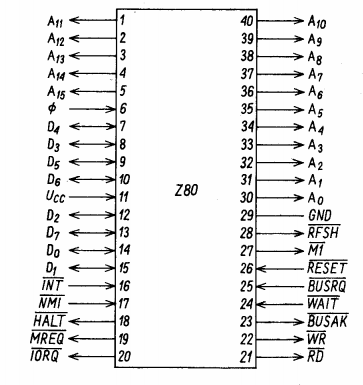
\includegraphics[width=1.0\textwidth]{z80wyprowadzenia}
		\caption{Wyprowadzenia mikroprocesora Z80}
		\label{img:z80wyprowadzenia}
	\end{figure}
	
	\subsection{Motywacja}
	
	\subsection{Aplikacja}
		
	\begin{figure}[h]		
		\centering
		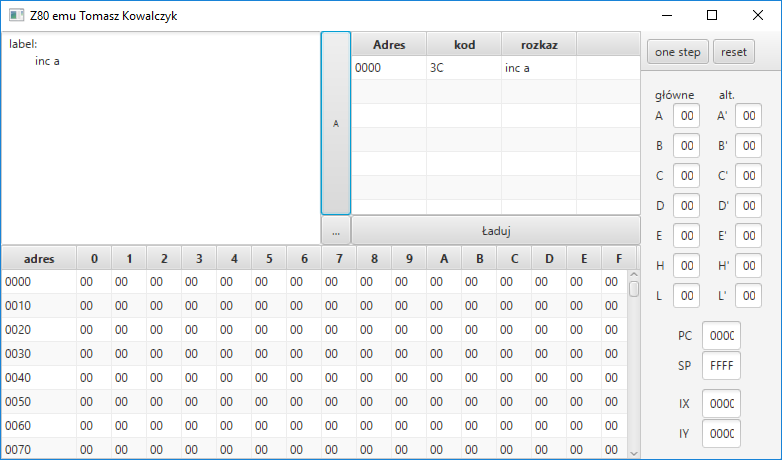
\includegraphics[width=1.0\textwidth]{app1}
		\caption{Widok główny emulatora}
	\end{figure}
	
	Interfejs użytkownika został podzielony na 3 części: 
	\begin{itemize}  
		\item widok kodu programu napisany w języku asembler, wraz z  wynikowym kodem maszynowym  
		\item widok pamięci w formie tabeli. Aby uzyskać adres odpowiadający danej komórce, należy dodać do siebie wartość \underline{?????}. Edycje wykonujemy przez dwukrotne kliknięcie w komórkę tabeli, wpisaniu nowej wartości i zatwierdzeniu klawiszem Enter.
		\item widok stanu wewnętrznych rejestrów procesora, wraz z przyciskami debugującymi.   
	\end{itemize}
	
	W aplikacji każda wyświetlona wartość podana jest w systemie heksadecymalnym, i także w takiej notacji wprowadzamy wartości (oprócz pola do edycji kodu asemblera, gdzie możemy używać innych notacji).
	
	\section{Zagadnienie emulacji}
	
	\subsection{różnica między symulacją a emulacją} 
	% Brakuje mi do tego bibliografii
	% linki z których czerpałem wiedze:
	% https://www.guru99.com/real-device-vs-emulator-testing-ultimate-showdown.html
	% http://fms.komkon.org/EMUL8/HOWTO.html
	% https://stackoverflow.com/questions/1584617/simulator-or-emulator-what-is-the-difference
	% https://www.quora.com/What-are-the-differences-between-simulation-and-emulation
	% TO NAJLEPSZE: https://softwareengineering.stackexchange.com/questions/134746/whats-the-difference-between-simulation-and-emulation
	Zagadnienie emulacji często mylone jest z symulacją. Nie są to jednak jednoznaczne pojęcia.
	
	W książe "Study of the techniques for emulation
	programming" Victor Moya del Barrio podaje taką to definicje emulatora "An emulator tries to duplicate the behaviour of a full computer using software programs in a different computer. "\cite{studyofthetechniquesforemulationprogramming}
		
		
%	Emulacja urządzenia, to próba naśladowania jego wewnętrznych mechanizmów. W przypadku mikroprocesora może to być odwzorowanie jego rejestrów wewnętrznych, liczników, magistral. Natomiast symulacja to imitacja funkcji urządzenia, nie skupia się na jego wewnętrznych stanach a tylko na zewnętrznych możliwościach. 
		
	% http://www.xsim.com/papers/Bario.2001.emubook.pdf	
	Emulacje można przeprowadzić na różne sposoby:
	\begin{itemize}  
		\item emulacja przez interpretowanie
		\item emulacja przez statyczną re-kompilacje
		\item emulacja przez dynamiczną re-kompilacje
	\end{itemize} \cite{fms_komkon_org_howto}	
	
	\subsection{emulacja przez interpretowanie}
	\subsection{emulacja przez statyczną re-kompilacje}
	\subsection{emulacja przez dynamiczną re-kompilacje}
	
	\section{Przegląd istniejących rozwiązań}
	Żadne istniejące rozwiązanie nie pozwala na podejrzenie wewnętrznych magistrali procesora
	
	\section{Projekt aplikacji}
	?????
	
	\section{Implementacja}
	Treść
	
	\section{Testy}
		
	\subsection{????}
	Bardzo ważną kwestią w projekcie było dokładne pokrycie kodu aplikacji w testach jednostkowych. Emulator mikro-kontrolera to specyficzna aplikacja. Z pozoru mało znaczący błąd może sprawić że emulator stanie się bezużyteczny. 
	
	Dla przykładu, jeśli dla 3 bajtowego rozkazu procesora zwiększymy rejestr PC o 2 zamiast o 3, to nie wykona się następna instrukcja przewidziana przez programistę. Dalsza praca emulatora stanie się nieprzewidywalna, a następna instrukcja całkowicie “wykolei” nasz program który zacznie wykonywać losowe instrukcje. 
	
	Dlatego poprawne wykonanie każdego rozkazu jest tak ważne dla mojego projektu. Aby uchronić się przed tego typu prostymi błędami każdy emulowany rozkaz posiada swój test/testy jednostkowe napisane przy pomocy biblioteki Junit. 
	
	Przykładowy test dla rozkazu LD A, I. Rozkaz ten ładuje zawartość rejestru A z I:
	\lstinputlisting[language=Java]{listings/exampleTest.java}
	
	Opisany przykład ukazuje że prosta z pozoru operacja jak pobranie wartości jednego rejestru i przeniesienie go do innego, wymaga objętościowych testów. Oprócz testowania czy poprawna wartość znajduje się w rejestrze docelowym, musimy sprawdzić także czy flagi CPU zostały ustawione na poprawnych wartościach, czy ilość przewidywanych cykli zegara została poprawnie zwiększona, czy rejestr PC został zainkrementowany. 
	
	\subsection{Test-driven development}
	TDD to metoda pisania oprogramowania. Zakłada ona że test jednostkowy dla danej funkcjonalności powstaje jako pierwszy. Dopiero po napisaniu testu implementujemy kod programu, a następnie testujemy za pomocą już napisanych testów. Za pomocą TDD była pisana cała aplikacja
	
	\section{Uwagi i wnioski}
	Treść
	
	\begin{thebibliography}{9}
		\bibitem{studyofthetechniquesforemulationprogramming}
		Victor Moya del Barrio
		\emph{Study of the techniques for emulation programming}.
		2001
		
		\bibitem{fms_komkon_org_howto}
		http://fms.komkon.org/EMUL8/HOWTO.html
		
		\bibitem{karczmarczuk}
		Mikroprocesor Z80 Jerzy Karczmarczuk
		
		\bibitem{manual} Oficjalny manual
	\end{thebibliography}
	
\end{document}